\documentclass{beamer}
% Copyright 2008  by Daina Chiba  <daina.chiba@gmail.com>
%
% This file can be redistributed and/or modified under
% the terms of the GNU Public License, version 2.

% Example presentation template file for beamerthemeRice version 0.02 (2008/11/22)

%===============================================================%
\mode<presentation> %use <handout> for handout mode
{
%\usetheme[compress, ricet, numbers]{Rice}
%\usetheme[ricet, smoothb]{Rice}
\usetheme[riceb, minimal]{Rice}
	% [ricet]		show the \Large "RICE" word mark at the top-right
	% [ricetm]		show the \large "RICE" word mark at the top-right
	% [ricets]		show the \small "RICE" word mark at the top-right
	% [riceb]		show the "RICE" word mark at the bottom-left
	% [compress]	show only the current section / subsection in the top navigation area.
	%			recommended if you have more than three subsections in at least one section
	% [minimal]	hide top navigation
	% [numbers]	show page numbers at the bottom-right
	% [noshadow]	remove shadow
	% [nologo]	remove Rice logo from the title page
	% [ricegray]	use ricegray instead of riceblue
	% [bgricegray]	use ricegray as background color
	% [bggray]	use light gray as background color
	% [smoothb]	top navigation with balls
\usefonttheme[onlymath]{serif}
	% \useoutertheme{infolines}
\setbeamercovered{transparent}
}
% In case you want to use other themes with riceblue...
%\usetheme{Frankfurt}
% AnnArbor, Antibes, Berlin, Berkeley, Bergen, Boadilla, boxes, CambridgeUS, Copenhagen
% Darmstadt, Dresden, Frankfurt
%\usecolortheme{riceowl}

\usepackage[english]{babel}
\beamerdefaultoverlayspecification{<+->}

\usepackage{mathptmx}
\usepackage{helvet}
\usepackage{courier}
% \usepackage{arev}
\usepackage[T1]{fontenc}
\usepackage{trajan}
\usepackage{animate}
\logo{
\includegraphics[width=20mm,scale=0.10]{Plots/redditlogo}}
%===============================================================%
\title[Meme Propagation]{Meme Propagation Through Reddit}

\author[]{James~Chen \\ Hoik~Jang \\ Steven~Oliver \\ Adrian~Perez}

%\institute
%{
%  Department of Statistics
%}

\subject{Beamer}


\begin{document}

% Comment out the following to remove the header & footer from the title page
% \thispagestyle{empty} 

\begin{frame}
 \titlepage
\end{frame}

\begin{frame}<beamer>
  \frametitle{Outline}
  \tableofcontents
\end{frame}

\section{Background} % Introduction

\subsection{Reddit} % Reddit

\begin{frame}{Reddit: "The Front Page of the Internet"}

Reddit operates as a collection of over a million communities known as \textit{subreddits}.
These are message boards oriented around a topic of interest such as:
\begin{center}
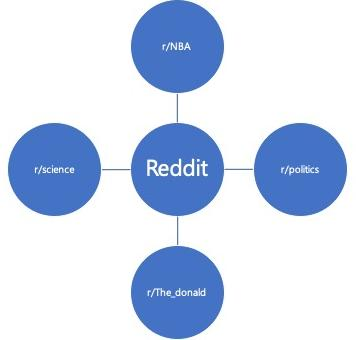
\includegraphics[scale=0.5]{Plots/redditsub}
\end{center}
Users interact within the subreddits by:
\begin{itemize}
\item posting content (images, gifs, or text discussion)
\item commenting on posts
\item voting
\end{itemize}

\end{frame}

\subsection{Summary Statistics} % Overview
\begin{frame}{Summary Statistics}
\begin{itemize}
	\item Data size: 6 months of data. On average, each month contains 70 Million Rows with 12 columns. 
	\item File type: JSON
	\item Process: Convert JSON in to SQL Database, then create subtables tables
	\item Established server
\end{itemize}
\end{frame}

\section{Objectives}

\subsection{Motivation} % Motivation
% Why is this important/interesting?
\begin{frame}{Motivation}
Reddit is one of the largest communities on the internet for new, revolutionary, and influential purposes. \\ User interaction within popular subreddits can have a great influence across the communities. Due to the richness and size of the dataset, we have proposed the following objectives:
\end{frame}




\subsection{Objectives}

\begin{frame}{Objectives}

\begin{block}<+->{Objective 1} 
Investigate relationships of the top 100 most active subreddits by tracking the spread of memes across those communities.
\end{block}

\begin{block}<+->{Objective 2} 
Analyze patterns of user comment activity in a multi-month span on Reddit.
\end{block}

\begin{block}<+->{Objective 3}
Analyze the fluctuations of user activity across subreddits by time of day.
\end{block}
\end{frame}

\section{Results} % Results

\subsection{Comment Activity}
\begin{frame}{Comment Activity}
\begin{columns}
    \begin{column}{0.4\textwidth}
        \begin{itemize}
            \item Time is in UTC (+6:00 CST)
            \item Users are from the US
            \item Peak activity during Lunch and 9pm
            \item Expected more night activity, can be due to young use age
        \end{itemize}
    \end{column}
    \begin{column}{0.75\textwidth}
        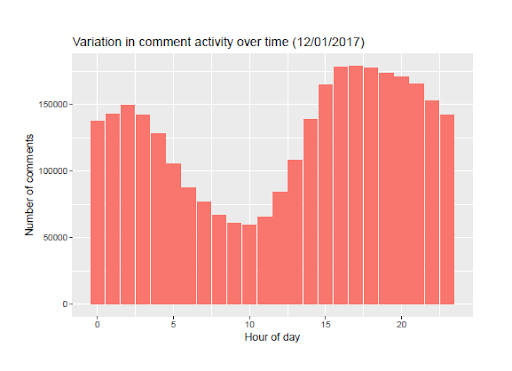
\includegraphics[width=\textwidth]{Plots/commentactivity}
    \end{column}
\end{columns}
\end{frame}


\subsection{Subscriber and Comment Counts}
\begin{frame}{Subscriber and Comment Counts}
\begin{columns}
    \begin{column}{0.40\textwidth}
        \begin{itemize}
            \item Expected decay with top subreddits
            \item Anomaly is explained by auto subscriptions
            \item Breaks linear regression pattern as well
        \end{itemize}
    \end{column}
    \begin{column}{0.70\textwidth}
        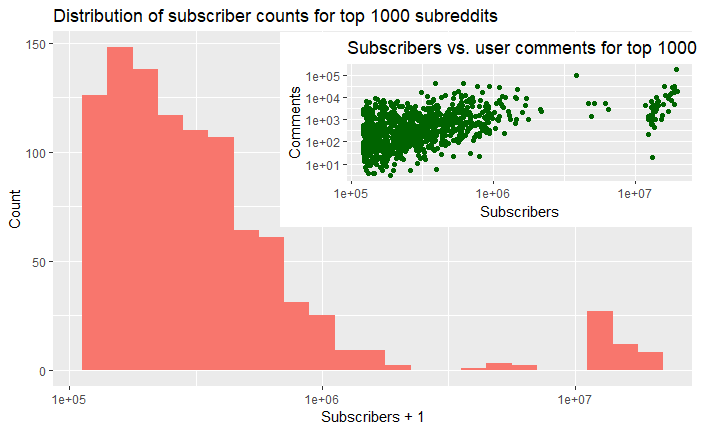
\includegraphics[width=\textwidth]{Plots/inset}
    \end{column}
\end{columns}
\end{frame}



\subsection{Danielle Meme}
\begin{frame}{Danielle}
\begin{center}
    
\includegraphics[width=\textwidth]{Plots/Danielle}
\end{center}
\end{frame}


\subsection{The Killer Plot}

\begin{frame}{The Killer Plot}
\begin{center}
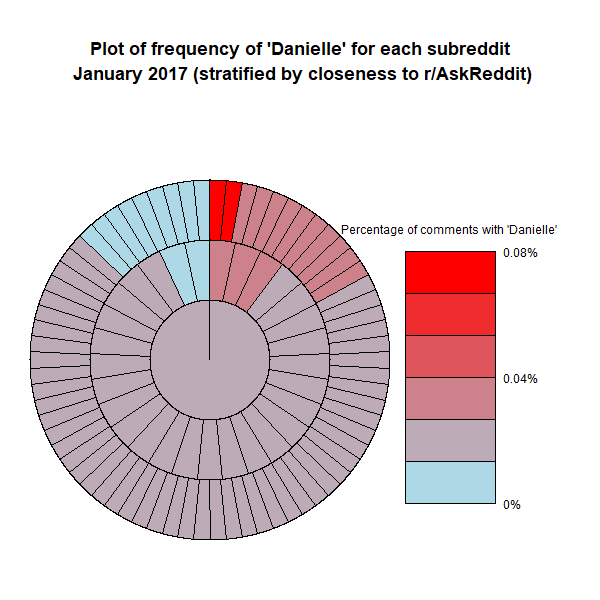
\includegraphics[width=8.5cm,scale=1]{Plots/janmemes}
\end{center}
\end{frame}

\begin{frame}{The Killer Plot}
\begin{center}
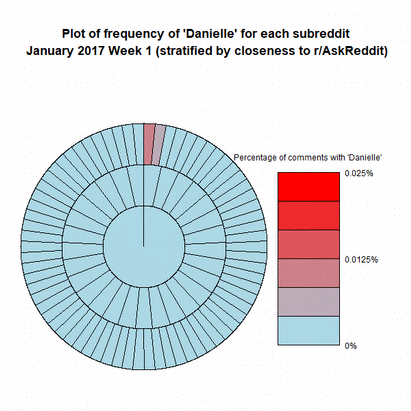
\includegraphics[width=8.5cm,scale=1]{Plots/2017_jan_week1}
\end{center}
\end{frame}

\begin{frame}{The Killer Plot}
\begin{center}
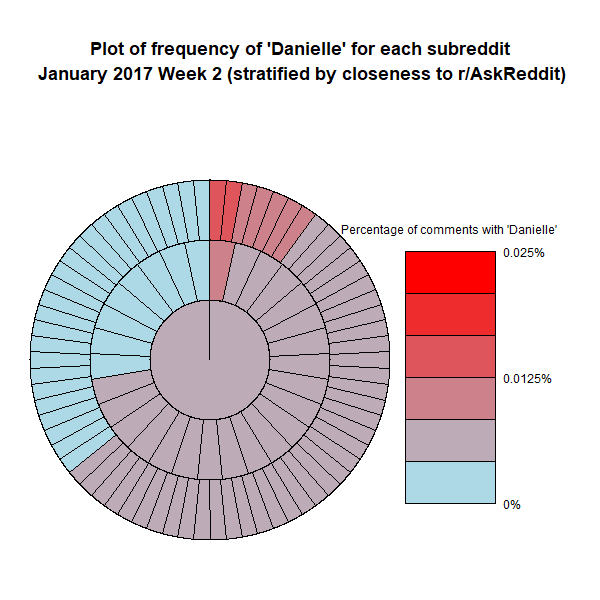
\includegraphics[width=8.5cm,scale=1]{Plots/2017_jan_week2}
\end{center}
\end{frame}

\begin{frame}{The Killer Plot}
\begin{center}
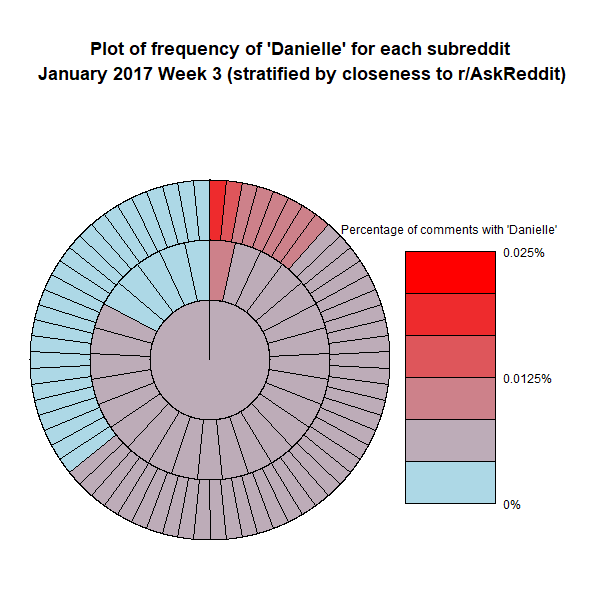
\includegraphics[width=8.5cm,scale=1]{Plots/2017_jan_week3}
\end{center}
\end{frame}

\begin{frame}{The Killer Plot}
\begin{center}
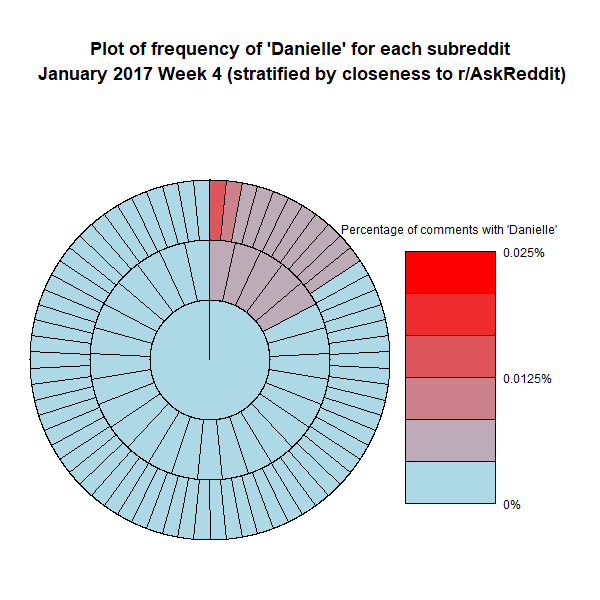
\includegraphics[width=8.5cm,scale=1]{Plots/2017_jan_week4}
\end{center}
\end{frame}

\begin{frame}{The Killer Plot}
\begin{itemize}
	\item Center is r/AskReddit, largest subreddit, and one of the first that Danielle meme appeared in
	\item Inner ring is 29 sibreddits most closely realted to r/AskReddit, based on cross-commenting activity
	\item Outer ring is 70 other subreddits less closely related to r/AskReddit
	\item Color scale is saturation percent of comments (percentage of comments containing the meme)
\end{itemize}
\end{frame}

\section{Conclusion}
\begin{frame}{Conclusion}
Takeaways:
\begin{itemize}
	\item Meme started in week 1, grew in weeks 2 and 3. and started dying off in week 4
	\item Two subreddits with most saturation of meme where in least correlation subreddits
	\begin{itemize}
		\item r/MMA
		\item r/hiphopheads
	\end{itemize}
	\item r/MMA might be the real center of the meme's spread
\end{itemize}
Future directions:
\begin{itemize}
	\item Should check with r/MMA but SQL queries take a while to run!
	\item Try this with more meme in other months (convfefe,Nothing but Respet for MY President).
\end{itemize}

\end{frame}

\end{document}
